\documentclass[landscape]{article}

\usepackage{tikz}
\usetikzlibrary{shapes, arrows}
\usepackage{amsmath}
\newcommand{\mx}[1]{\mathbf{\bm{#1}}} % Matrix command
\newcommand{\vc}[1]{\mathbf{\bm{#1}}} % Vector command
\usepackage{geometry}
 \geometry{
 a4paper,
 total={170mm,257mm},
 left=5mm,
 top=5mm,
 bottom=5mm,
 }

\begin{document}

% define the layers to draw the diagram
\pgfdeclarelayer{background}
\pgfdeclarelayer{foreground}
\pgfsetlayers{background,main,foreground}

% define block styles used later
\tikzstyle{image} = [inner sep=0pt]
\tikzstyle{label} = [rectangle, align=center, text width=2cm, font=\bfseries]
\tikzstyle{arrow} = [thick,->,>=stealth, line width=0.8mm]

\begin{tikzpicture}[line width=0.5mm, node distance=0pt]
    \pagenumbering{gobble}
    
    \node (c1) [label] {RGB frames};
    \node (i1_1) [image, right of=c1, xshift=0.18\textwidth] {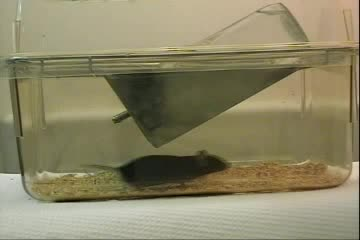
\includegraphics[width=.2\textwidth]{images/tvl1/r/w1.jpg}};
    \node (i1_2) [image, right of=i1_1, xshift=0.205\textwidth] {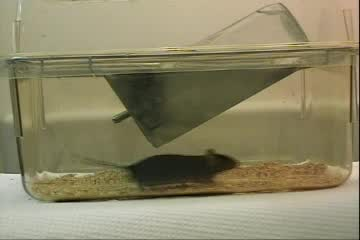
\includegraphics[width=.2\textwidth]{images/tvl1/r/w2.jpg}};
    \node (i1_3) [image, right of=i1_2, xshift=0.205\textwidth] {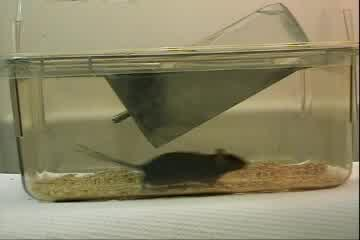
\includegraphics[width=.2\textwidth]{images/tvl1/r/w3.jpg}};
    \node (i1_4) [image, right of=i1_3, xshift=0.205\textwidth] {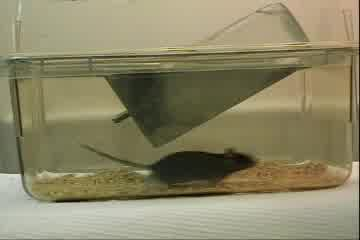
\includegraphics[width=.2\textwidth]{images/tvl1/r/w4.jpg}};
    \node (i1_5) [image, right of=i1_4, xshift=0.205\textwidth] {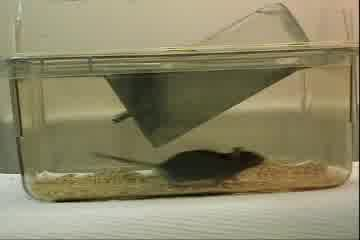
\includegraphics[width=.2\textwidth]{images/tvl1/r/w5.jpg}};
    \node (i1_6) [image, right of=i1_5, xshift=0.205\textwidth] {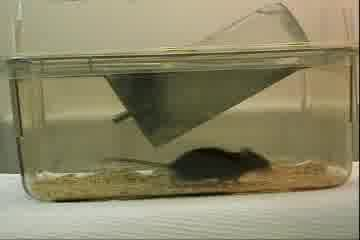
\includegraphics[width=.2\textwidth]{images/tvl1/r/w6.jpg}};
    \node (i1_7) [image, right of=i1_6, xshift=0.205\textwidth] {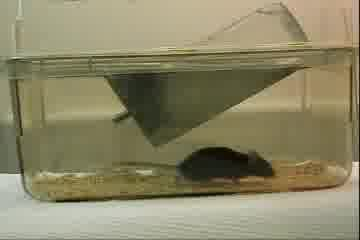
\includegraphics[width=.2\textwidth]{images/tvl1/r/w7.jpg}};

    \node (c2) [label, below of=c1, yshift=-6cm] {u-channel\\ frames};
    \node (i2_1) [image, right of=c2, xshift=0.18\textwidth] {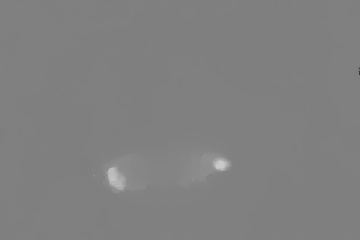
\includegraphics[width=.2\textwidth]{images/tvl1/u/w1.jpg}};
    \node (i2_2) [image, right of=i2_1, xshift=0.205\textwidth] {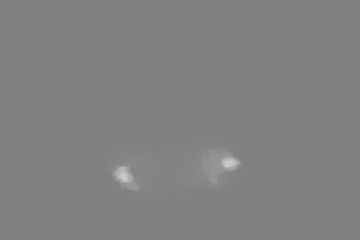
\includegraphics[width=.2\textwidth]{images/tvl1/u/w2.jpg}};
    \node (i2_3) [image, right of=i2_2, xshift=0.205\textwidth] {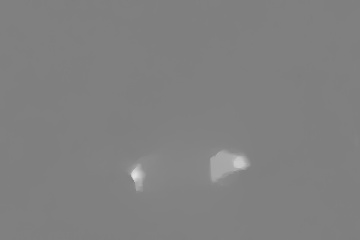
\includegraphics[width=.2\textwidth]{images/tvl1/u/w3.jpg}};
    \node (i2_4) [image, right of=i2_3, xshift=0.205\textwidth] {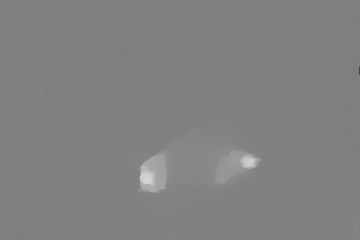
\includegraphics[width=.2\textwidth]{images/tvl1/u/w4.jpg}};
    \node (i2_5) [image, right of=i2_4, xshift=0.205\textwidth] {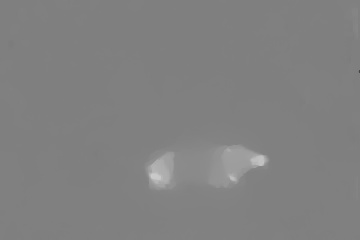
\includegraphics[width=.2\textwidth]{images/tvl1/u/w5.jpg}};
    \node (i2_6) [image, right of=i2_5, xshift=0.205\textwidth] {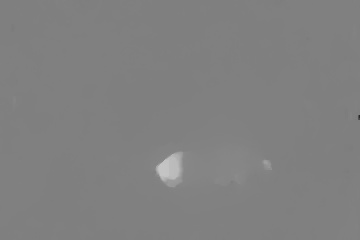
\includegraphics[width=.2\textwidth]{images/tvl1/u/w6.jpg}};
    \node (i2_7) [image, right of=i2_6, xshift=0.205\textwidth] {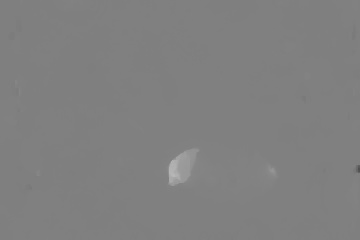
\includegraphics[width=.2\textwidth]{images/tvl1/u/w7.jpg}};

    \node (c3) [label, below of=c2, yshift=-3cm] {v-channel\\ frames};
    \node (i3_1) [image, right of=c3, xshift=0.18\textwidth] {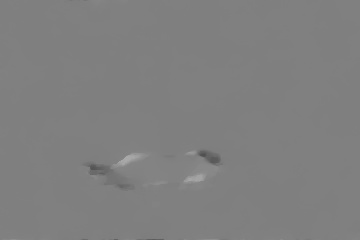
\includegraphics[width=.2\textwidth]{images/tvl1/v/w1.jpg}};
    \node (i3_2) [image, right of=i3_1, xshift=0.205\textwidth] {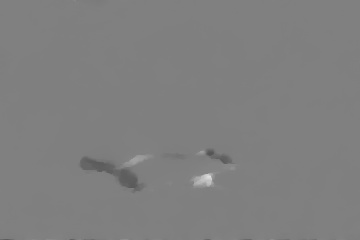
\includegraphics[width=.2\textwidth]{images/tvl1/v/w2.jpg}};
    \node (i3_3) [image, right of=i3_2, xshift=0.205\textwidth] {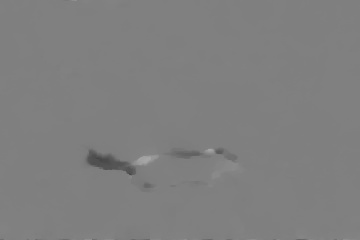
\includegraphics[width=.2\textwidth]{images/tvl1/v/w3.jpg}};
    \node (i3_4) [image, right of=i3_3, xshift=0.205\textwidth] {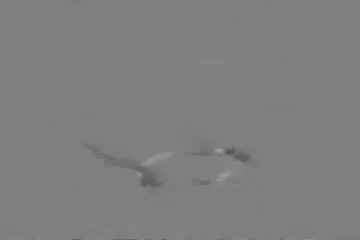
\includegraphics[width=.2\textwidth]{images/tvl1/v/w4.jpg}};
    \node (i3_5) [image, right of=i3_4, xshift=0.205\textwidth] {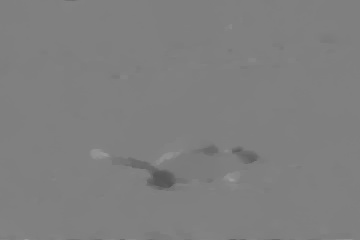
\includegraphics[width=.2\textwidth]{images/tvl1/v/w5.jpg}};
    \node (i3_6) [image, right of=i3_5, xshift=0.205\textwidth] {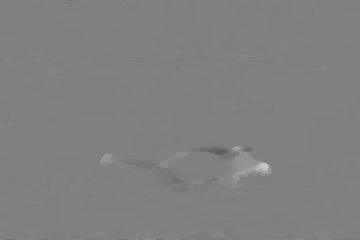
\includegraphics[width=.2\textwidth]{images/tvl1/v/w6.jpg}};
    \node (i3_7) [image, right of=i3_6, xshift=0.205\textwidth] {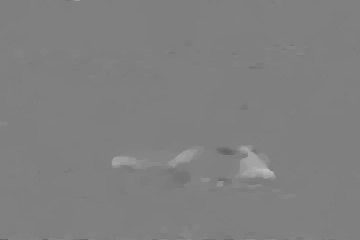
\includegraphics[width=.2\textwidth]{images/tvl1/v/w7.jpg}};

    \path (i2_1.west |- i2_1.north)+(-2.3,+1) node (a) {};
    \path (i3_7.east |- i3_7.south)+(+0.5,-0.6) node (c) {};          
    \path [rounded corners, draw=black!255, line width=1pt] (a) rectangle (c);

    \node (op) [label, right of=a, xshift=1.6cm, yshift=-0.5cm, text width=3cm] {\Large Optical flow};

    \path (i1_4.west |- i1_4.south)+(1,0) node (x) {};
    \path (i2_4.west |- i2_4.north)+(1,1) node (y) {};
    \draw [arrow] (x) to node[anchor=west] {\textbf{  TVL1} Algorithm} (y);

\end{tikzpicture}

\end{document}